\chapter{Der QHScompiler} \label{cha:4-QHS_Compiler}
Der QHScompiler basiert auf einem von mir erdachten alternativen Aufbau für einen Compiler. Diesem Aufbau liegt eine einfache Idee zugrunde:
Die Macros die der Macro Expansion aus Abschnitt \ref{sec:traditional_code_generation} sollen erst während der Kompilierung definiert werden. 
Auf dieser Grundidee werde ich zwei Dinge aufbauen. Erstens halte ich es für möglich, mit der richtigen Verwendung von Macros die gesammte syntaktische Analyse zu überspringen und keinen AST generieren zu müssen.
Zweitens sollte es rein durch die Veränderung von diesen Macros möglich sein jegliche Programmiersprache zu kompilieren. Man könnte also in einem Dokument verschiedene Programmiersprachen verwenden und
müsste dazwischen bloss die jeweiligen Macros neu definieren. Das selbige gilt ebenfalls für die Ausgabesprache.
Nur durch das Umdefinieren der Macros liesse sich die Ausgabesprache wechseln, ohne eine Änderung am Compiler vornehmen zu müssen.
Um dies zu verwirklichen, folgt mein alternativer Ansatz einem Aufbau, der sich stark von einem traditionellen Compiler unterscheidet.

Die Programmiersprache, in der sich meine Macros definieren lassen, bezeichne ich als QHS. Der Compiler der QHS versteht und kompiliert, nenne ich dazu passend den QHScompiler.
QHS besteht wie die meisten anderen Programmiersprachen aus Wörtern. Im Kontext von QHS werden diese Wörter \textit{Orders} genannt.
Orders können drei verschiedenen Typen aufweisen: \textit{Identifiers}, \textit{Instructions} und \textit{LiteralCode}.
%Bei Identifiers handelt es sich um die bereits erwähnten Macros, Instructions sind einfache vorprogrammierte Anweisungen an den QHScompiler und LiteralCode ist Text, der unverändert in die Ausgabedatei geschrieben wird.
Wie diese drei Ordertypen genau funktionieren, wird in Abschnitt \ref{sec:qhs-execute} ausführlicher erklärt.

Der Kompilierung durch den QHScompiler steht ein einfacher Zyklus zugrunde, dessen Inspiration der Von-Neumann Zyklus ist.

\begin{figure}[h!]
    \centering
    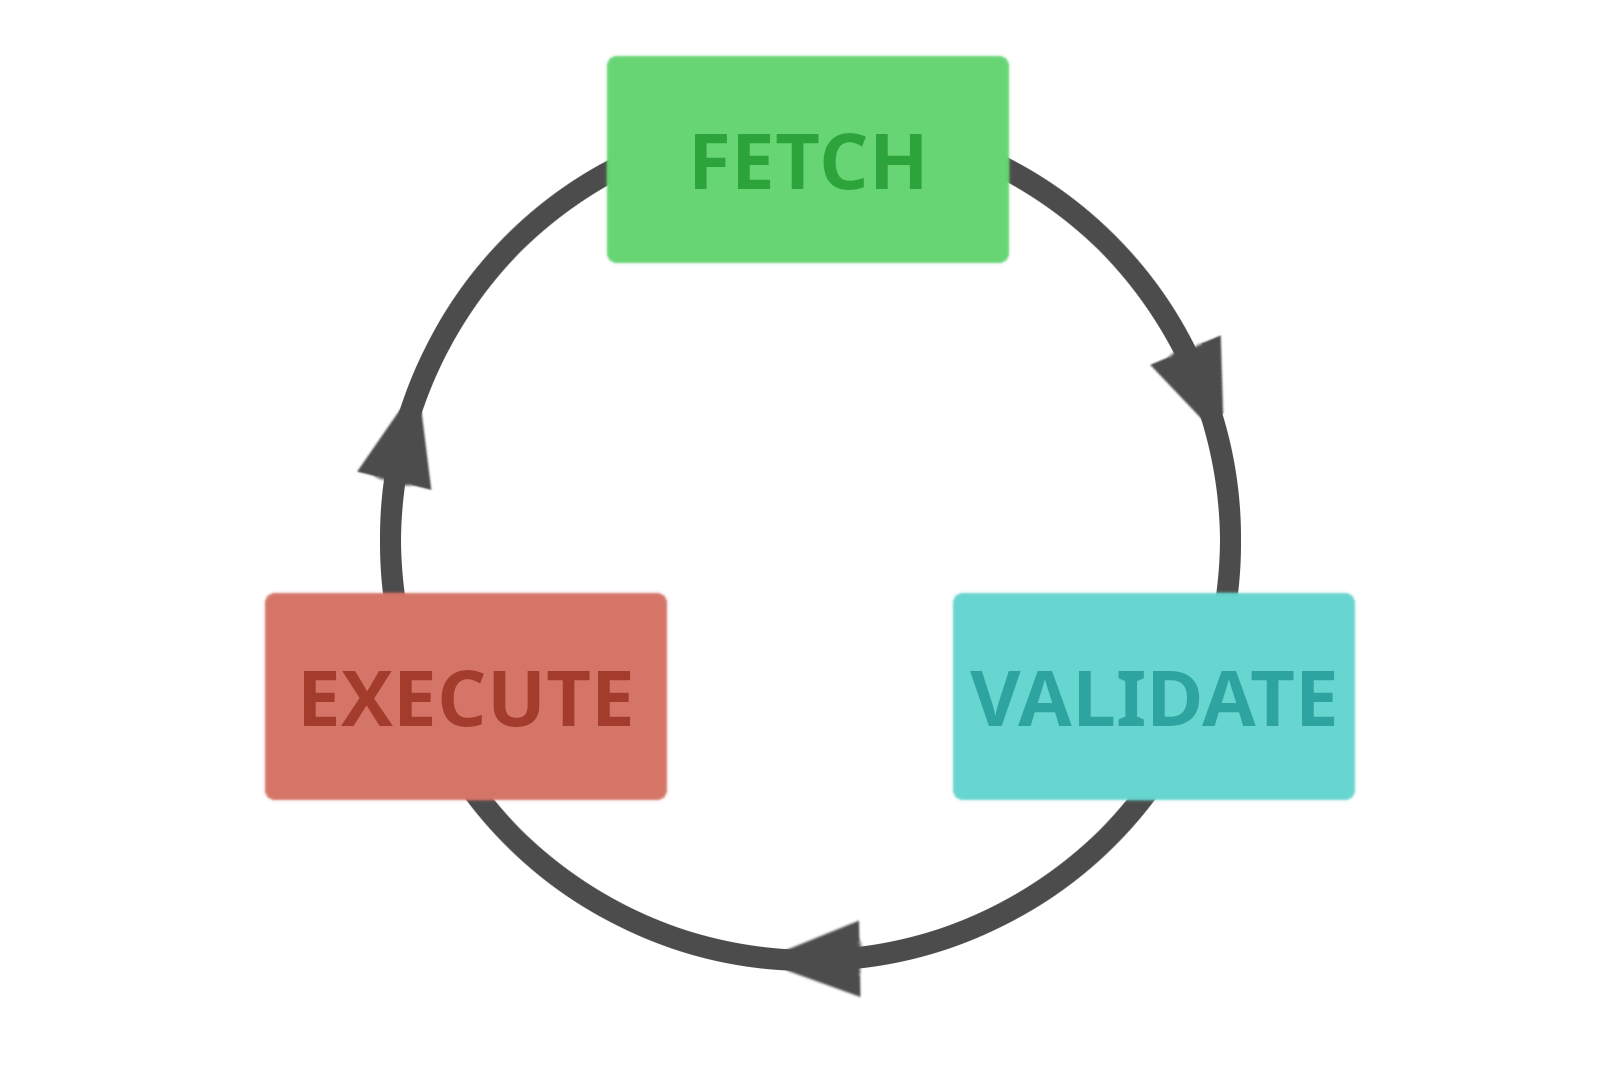
\includegraphics[scale=0.6]{resources/images/qhs-cycle.png}
    \caption{Zyklus der QHS Kompilierung (QHS-Zyklus)}
    \label{fig:qhs-cycle}
\end{figure}

\section{Die Fetch-Phase} \label{sec:qhs-fetch}
Die Aufgabe der \textit{Fetch-Phase} ist es die nächste \textit{Order}, die verarbeitet werden soll, zu finden. In dieser Hinsicht gleicht die Fetch-Phase der lexikalische Analyse eines traditionellen Compilers.
Der QHS-Zyklus beginnt bei der Fetch-Phase, dabei wird die erste \textit{Order} aus der Eingabedatei extrahiert. In jeder weiteren Fetch-Phase wird die nächste \textit{Order} aus der Eingabedatei geholt.
Die Fetch-Phase ist auch dafür zuständig die nächste \textit{Order} einem der drei Typen (Identifier, Instruction oder LiteralCode) zuzuordnen.
Diese \textit{Ordertypen} sind mit folgenden Regular Expressions definiert. Leerzeichen dienen als Trennung zwischen \textit{Orders} und werden ignoriert.

\begin{table}[h]
    \centering
    \caption{RegEx Definitionen der \textit{Ordertypen}}
    \vspace{3mm} % Adjust the height of the space between caption and tabular
    
    \begin{tabular}{ll}
    \multicolumn{1}{l|}{identifier}        & \textless{}identiferChar\textgreater{}+                           \\ \hline
    \multicolumn{1}{l|}{instruction}       & \# \textless{}identiferChar\textgreater{}+                        \\ \hline
    \multicolumn{1}{l|}{literalCode}       & ".*"                                                              \\
                                           &                                                                   \\
    \textless{}identiferChar\textgreater{} & = {[}\textasciicircum{}\# "\textless{}whitespace\textgreater{}{]} \\
    \textless{}whitespace\textgreater{}    & = SPACE | NEWLINE | TAB
    
    \end{tabular}
\end{table}

Im Vergleich zu traditionellen Compilern fällt auf, dass beim QHScompiler kaum zwischen Zeichen differenziert wird. Während die lexikalische Analyse traditionell zwischen vielen verschiedenen Tokens unterscheidet,
sind für den QHScompiler alle Zeichen (mit Ausnahme von \# und ") gleichbedeutend.

Normalerwiese erhält die Fetch-Phase die nächste \textit{Order} aus der Eingabedatei. 
Es ist jedoch möglich \textit{Orders} der Eingabedatei voranzustellen. Diese \textit{Orders} werden in der Fetch-Phase zuerst gefunden. Dies geschieht mithilfe des \textit{FetchStacks}, auf den \textit{Orders} gelegt werden können.
In der nächsten Fetch-Phase wird immer die oberste \textit{Order} des FetchStacks geholt und daraufhin vom FetchStack entfernt.
Die Eingabedatei befindet sich auf dem untersten Platz des FetchStacks und wird somit nur verwendet, wenn der Stack ansonsten komplett leer ist.
%Eine \textit{Order} kann während jedem der drei Schritte des QHS-Zyklus auf den FetchStack gelegt werden.

FETCHSTACK FIGURE

%Während der Laufzeit des QHScompilers könnte der FetchStack folgendermassen aussehen:
%
%\begin{figure}[h!]
%    \centering
%    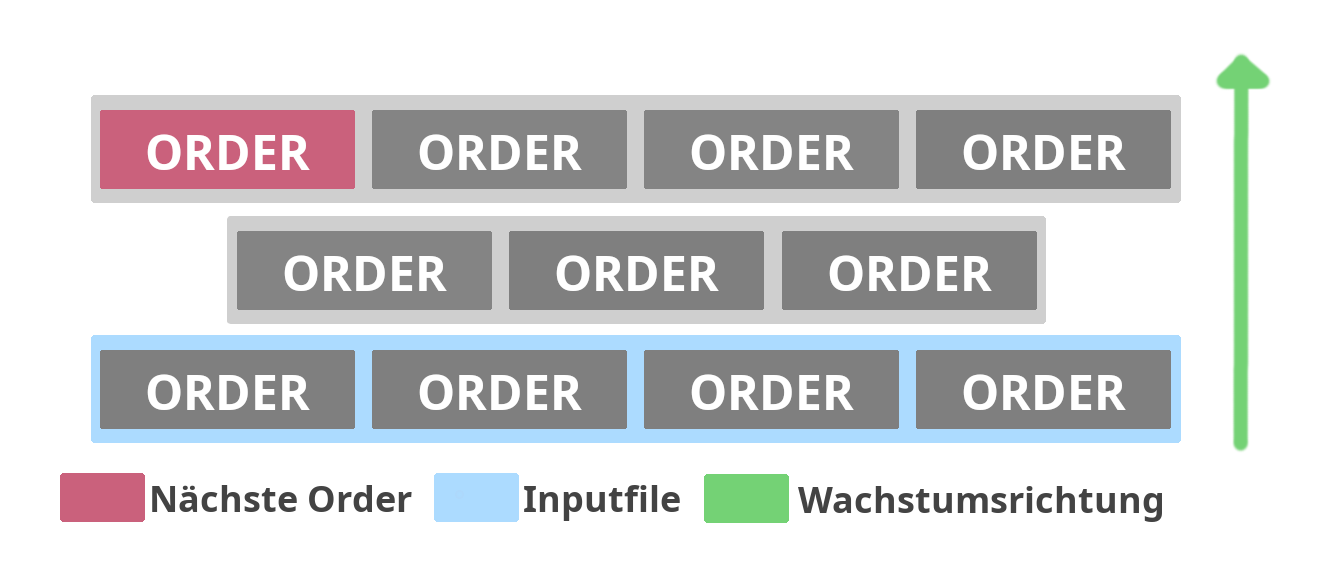
\includegraphics[scale=1.1]{resources/images/fetch-stack.png}
%    \caption{Struktur des FetchStacks UPDATE}
%    \label{fig:fetchstack}
%\end{figure}
%
Die Hauptanwendung des FetchStacks wird im Abschnitt \ref{sec:qhs-execute} erklärt.
Die Kompilierung ist beendet, sobald keine \textit{Order} mehr auf dem FetchStack vorhanden ist.

\section{Die Validate-Phase} \label{sec:qhs-Validate}
Nachdem die nächste \textit{Order} in der  Fetch-Phase gefunden wurde, wird diese \textit{Order} an die Validate-Phase weitergegeben. Während der Validate-Phase kommt die \textit{OrderQueue} ins Spiel.
Dabei handelt es sich, wie der Name schon sagt, um eine Queue von \textit{Orders}.
Die Aufgabe der \textit{OrderQueue} ist das Speichern und spätere Zurückholen von \textit{Orders}. Die \textit{OrderQueue} kann mit Instructions, die im Abschnitt \ref{sec:qhs-execute} weiter ausgeführt werden, aktiviert und deaktiviert werden.
Wenn eine \textit{Order} in die Validate-Phase gelangt und die \textit{OrderQueue} aktiviert ist, wird diese \textit{Order} der \textit{OrderQueue} hinzugefügt.
Die Execute-Phase wird danach übersprungen und der QHS-Zyklus beginnt von neuem bei Fetch.
Die \textit{Order} wurde (ohne die Execute-Phase erreicht zu haben) auf der \textit{OrderQueue} gespeichert. Später ist es mit Instructions möglich diese \textit{Order} von der \textit{OrderQueue} zu entfernen und auszuführen.

Bestimmte \textit{Orders} können jedoch \textit{orderQueue-proof}, also immun gegen die \textit{OrderQueue}, gemacht werden.
\textit{Orders}, die \textit{orderQueue-proof} sind, werden an die Execute-Phase weitergegeben, auch wenn die \textit{OrderQueue} aktiv ist.
Dieses Prinzip ist zum Beispiel besonders bei der Instruction, welche die \textit{OrderQueue} wieder deaktiviert, wichtig.
Da diese Instruction ansonsten nicht zur Execute-Phase gelänge und somit die \textit{OrderQueue} nie deaktiviert würde.
Zu beachten ist, dass LiteralCode nicht \textit{orderQueue-proof} sein kann.

MAYBE CODESTACK FIGURE

Ist die \textit{OrderQueue} deaktiviert oder die \textit{Order} \textit{orderQueue-proof}, wird diese \textit{Order} an den letzten Schritt Execute weitergegeben.

\section{Die Execute-Phase} \label{sec:qhs-execute}
Während der Execute-Phase wird der tatsächliche Assembly Code generiert. Je nach Typ der \textit{Order} (Identifier, Instruction oder LiteralCode) läuft die Execute-Phase sehr unterschiedlich ab.
In den folgenden Abschnitten wird der Ablauf der Execute-Phase je nach \textit{Ordertyp} erklärt.

\subsection{Identifier}
Identifier stehen für die am Anfang von Abschnitt \ref{cha:4-QHS_Compiler} erwähnten Macros. Diese Identifier sind in einem \textit{Environment} definiert.
Bei einem Environment handelt es sich um eine einfache Map, die einen Identifier mit einer Liste an \textit{Orders} verknüpft.
%In anderen Programmiersprachen werden Environments auch als Scope bezeichnet.
Wenn nun ein Identifier in die Execute-Phase gelangt, werden die dazugehörigen \textit{Orders} auf den FetchStack aus Abschnitt \ref{sec:qhs-fetch} gelegt.
Bei den nächsten Fetch-Phasen werden nun zuerst die zum Identifier gehörenden \textit{Orders} nacheinander abgebaut. Einfach ausgedrückt wird der Identifier also durch seine \textit{Orders} ersetzt.

EXAMPLE FIGURE?

Die bereits erwähnten Environments sind dabei in einer Linked-List gespeichert. Somit können neue Environments zu dieser Liste hinzugefügt und aus der Liste entfernt werden.
Das letzte Environment der Liste ist das älteste und das erste Environment das neuste.
Ein neuer Identifier wird immer zum ersten Environment hinzugefügt. Definitionen des gleichen Identifiers in älteren Environments werden nicht überschrieben oder gelöscht.
Bei der Abfrage nach einem Identifier wird immer die neuste vorhandene Definition zurückgegeben. Ist keine vorhanden, wird ein Error ausgegeben.

\subsection{Instructions}
%Instructions sind die komplexesten \textit{Orders} für die Execute-Phase. 
Wenn eine Instruction in die Execute-Phase gelangt, wird die dazu definierte Funktion im QHScompiler ausgeführt.
Diese Funktionen können Variablen im QHScompiler speichern, die \textit{OrderQueue} aktivieren, Identifier definieren und vieles mehr. Instructions sind somit der Weg wie während der Kompilierung auf den QHScompiler einfluss genommen werden kann.
In der Tabelle \ref{tab:important_instructions} sind ein paar der wichtigsten Instructions aufgelistet:

\begin{table}[H]
    \centering
    \caption{Wichtige Instructions des QHScompilers}
    \label{tab:important_instructions}
    \vspace{3mm} % Adjust the height of the space between caption and tabular
    
    \begin{tabularx}{\textwidth}{l|X}
    \textbf{Instruction}                             & \textbf{Beschreibung} \\ \hline
    {\listingFont\selectfont \#enterOrderQueue}      & Aktiviert die \textit{OrderQueue}. \\ \hline
    {\listingFont\selectfont \#exitOrderQueue}       & Deaktiviert die \textit{OrderQueue}. \\ \hline
    {\listingFont\selectfont \#assign}               & Die erste \textit{Order} der \textit{OrderQueue} muss ein Identifier sein. Der Rest der \textit{Orders} auf der \textit{OrderQueue} wird als Definition für diesen Identifier festgelegt. \\ \hline
    {\listingFont\selectfont \#assignToOne}          & Wie \#assign, jedoch wird nach dem Identifier nur eine weitere \textit{Order} von der \textit{OrderQueue} genommen und als Definition für den Identifier verwendet. \\ \hline
    {\listingFont\selectfont \#force}                & Die nächste \textit{Order} wird nach der Fetch-Phase sofort an die Execute-Phase weitergegeben. Überspringt Validate und somit die \textit{OrderQueue}. \\ \hline
    %{\listingFont\selectfont \#lightForce}           & Ähnlich wird \#force, jedoch wird diese nur ausgeführt, wenn \textbf{explain this cuz they don't know OrderQueue depth} \\ \hline
    {\listingFont\selectfont \#orderEnqueue}         & Die nächste \textit{Order} wird sofort dem Ende der \textit{OrderQueue} hinzugefügt, auch wenn diese \textit{Order} \textit{orderQueue-proof} wäre. Die Execute-Phase wird übersprungen. \\ \hline
    {\listingFont\selectfont \#orderFrontEnqueue}    & Ähnlich wie \#orderEnqueue. Die \textit{Order} wird jedoch an den ersten Platz der \textit{OrderQueue} gesetzt. \\ \hline
    {\listingFont\selectfont \#deepFetch}            & Die nächste \textit{Order} der Eingabedatei wird oben auf den FetchStack gesetzt. Ermöglicht den Zugriff auf die Eingabedatei innerhalb eines Identifiers. \\ \hline
    {\listingFont\selectfont \#queueFetch}           & Die erste \textit{Order} der \textit{OrderQueue} wird oben auf den FetchStack gesetzt. \\ \hline 
    {\listingFont\selectfont \#pushEnv}              & Ein neues Environment wird der Environment Linked-List hinzugefügt. \\ \hline
    {\listingFont\selectfont \#popEnv}               & Das neuste Environment der Environment Linked-List wird gelöscht. \\ \hline
    {\listingFont\selectfont \#addToIdentifier}      & Die erste \textit{Order} der \textit{OrderQueue} muss ein Identifier sein und die zweiterste LiteralCode. Beide \textit{Orders} werden als Zahl interpretiert und addiert.
                                                       Das Resultat wird im Identifier gespeichert.       
    \end{tabularx}
\end{table}

Der QHScompiler umfasst \textbf{33} Instructions, wobei \textbf{5} dieser ausschliesslich fürs Debuggen des Compilers dienen.

\subsection{LiteralCode}
LiteralCode ist der Weg wie der QHScompiler Assembly Code generiert. Dieser ist sehr einfach. Wenn LiteralCode in die Execute-Phase gelangt, wird alles, das zwischen den Satzzeichen steht, in die Ausgabedatei geschrieben.
Dies ist die einzige Möglichkeit des QHScompiler Assembly Code zu generieren. Einzig die \textit{LiteralCode-Orders} bestimmen, was in die Ausgabedatei gelangt, und somit welcher Sprache diese Ausgabedatei folgt. 
Durch das Anpassen der \textit{LiteralCode-Orders} ist es also möglich die Ausgabesprache des QHScompilers zu ändern.


\section{Definition der Macros} \label{sec:qhs-macro_definitions}
Somit ist der QHScompiler komplett. Grundsätzlich lässt sich mit QHS bereits jedes Programm schreiben und mit dem QHScompiler kompilieren. 
Jedoch habe ich in Tabelle \ref{tab:requirements} festgelegt, dass die Eingabesprache einen C ähnlichen Syntax aufweisen muss.
Um dies zu ermöglichen, muss man, wie zu Beginn von Abschnitt \ref{cha:4-QHS_Compiler} erwähnt, bestimmte Macros also Identifier definieren.
In diesem Abschnitt werde ich zeigen, wie sich diese Identifier auch für syntaktisch komplexe Programmiersprachen definieren lassen.
Zur Veranschaulichung dienen Variablen und Funktionsdefinitionen.


\iffalse
Der QHScompiler ist zwar komplett, die dazugehörige Programmiersprache QHS jedoch noch lange nicht.
Grundsätzlich ist es möglich mit LiteralCode jedes Programm zu schreiben und zu kompilieren, jedoch handelt es sich dann nur um Assembly Code.
Doch der Aufbau des QHScompilers ermöglicht es mit Identifiern eine komplexere Programmiersprache zu definieren. Ein fester Bestandteil ein jedes Programms, das mit dem QHScompiler kompiliert werden soll, ist ein Stück Code,
das die jeweilige Programmiersprache definiert. Dieser Code wird im Kontext des QHScompilers \textit{Preamble} genannt. Theoretisch ist es möglich durch das Anpassen dieses Preambles, 
viele unterschiedliche Programmiersprachen mit dem QHScompiler zu kompilieren. In diesem Abschnitt wird behandelt wie sich die Sprache QHS, welche die Kriterien aus Abschnitt \ref{sec:Vergleichs_Kriterien} erfüllt,
für den QHScompiler definieren lässt.
\fi

\subsection{Abkürzungen}
In diesem Abschnitt wird viel QHS-Code als Beispiel verwendet.
Um die Leserlichkeit von QHS zu verbessern, werden ein zuerst paar Identifier anstelle der umständlichen Instructions definiert.
Diese Identifier sind in der folgenden Tabelle \ref{tab:shortcuts} aufgeführt.

{
\begin{table}[H]
    \centering
    \caption{Identifier als Abkürzung von Instruction}
    \vspace{3mm} % Adjust the height of the space between caption and tabular
    \label{tab:shortcuts}
    
    \begin{tabular}{l|l}
    \textbf{Identifier}                                     & \textbf{Definition}            \\ \hline
    {\listingFont\selectfont [}                             & \#enterOrderQueue              \\ \hline
    {\listingFont\selectfont ]}                             & \#exitOrderQueue               \\ \hline
    {\listingFont\selectfont \textgreater{}\textgreater{}}  & \#assign                       \\ \hline
    {\listingFont\selectfont -\textgreater{}}               & \#assignToOne                  \\ \hline
    {\listingFont\selectfont !}                             & \#force                        \\ \hline
    %{\listingFont\selectfont ?!}                            & \#lightForce                   \\ \hline
    {\listingFont\selectfont \textbackslash{}n}             & Eine neue Zeile im Ausgabedatei
    \end{tabular}
\end{table}
}

Weiter wird innerhalb von Kommentaren Pseudo-Code verwendet, um den QHS Code verständlicher zu erklären.
Kommentare können mehrere Zeilen umfassen und beginnen immer mit {\listingFont\selectfont /*} und enden mit {\listingFont\selectfont*/}.
Der Kommentar {\listingFont\selectfont /* X = "hello" \#pushEnv */} würde bedeuten,
dass der Identifier {\listingFont\selectfont X} zu den \textit{Orders} {\listingFont\selectfont "hello" (LiteralCode)} und {\listingFont\selectfont \#pushEnv (Instruction)} definiert wurde. 

Auch wird bei längeren Identifier-Definitionen wird zuerst der zudefinierende Identifier getrennt von den restlichen \textit{Orders} der \textit{OrderQueue} hinzugefügt.
Diese Separation dient der besseren Leserlichkeit und hat keinen Einfluss auf die Kompilierung des Codes.

EXAMPLE

\subsection{Identifier Parameter und Rückgabewert}
Mit den \#enterOrderQueue (rsp. [ ) und \#exitOrderQueue (rsp. ] ) Instructions kann innerhalb eines Identifiers die \textit{OrderQueue} verwendet werden. Dies ermöglicht eine Art von Parameter und Rückgabewert für Identifier.
Parameter werden vor dem Aufruf eines Identifiers der \textit{OrderQueue} hinzugefügt. Diese können dann innerhalb des Identifiers verwendet werden.
Genauso kann der Identifier \textit{Orders} der \textit{OrderQueue} hinzufügen und diese somit zurückgeben.

\begin{lstlisting}[language=QHS, caption=Verwendung von Parametern und Rückgabewert eines Identifiers]
[ foo ]
[
    #orderFrontEnqueue param1 ->    /* param1 = erstes Argument */
    #orderFrontEnqueue param2 ->    /* param2 = zweites Argument */

    param1 " : " param2 \n          /* param1 + " : " + param2 + "\n" */

    [ "return" ]                    /* "return" wird der OrderQueue hinzugefügt */
] >>

[ "1" "2" ]                         /* 2 Argumente werden der OrderQueue hinzugefügt */
foo                                 /* foo wird ausgeführt */
#queueFetch                         /* Die zurückgegebene Order wird von der OrderQueue
                                    geholt und ausgeführt */


%\noindent\hrulefill Ausgabe\noindent\hrulefill%
1 : 2
return
\end{lstlisting}


\subsection{Variablen} \label{sec:qhs-vars}
Die Umsetzung von Variablen in QHS ist einfach.
Um Platz für die Variable auf dem Stack zu schaffen, muss zuerst die Grösse der Variable in Bytes vom rsp subtrahiert werden.
%Zuerst soll der Assembly Code für das Abziehen der Grösse der Variable vom Stack-Pointer hinzugefügt werden.
Dann wird für die Variable ein Identifier definiert, der zur Position der Variable auf dem Stack zeigt.
Mit LiteralCode lässt sich dies wie folgt in QHS ausdrücken:

\begin{lstlisting}[language=QHS, caption=Definition einer Variable mit LiteralCode]
"sub rsp, 4" \n
[ a "[rbp-4]" ] >>      /* a = "[rbp-4]" */

"add " a ", 5"

%\noindent\hrulefill Ausgabe\noindent\hrulefill%
sub rsp, 4
add [rbp-4], 5
\end{lstlisting}

Jedoch braucht man für diese Implementation immer noch viel LiteralCode und Assembly Kenntnisse. Um die Definition von Variablen C ähnlicher zu machen, lässt sich zum Beispiel ein \textit{var} Identifier definieren.
Dieser \textit{var} Identifier nimmt die Grösse der Variable als Argument über die \textit{OrderQueue} an. Um die in C geläufige Syntax der Definition einer Variable beizubehalten,
wird der Name der Variable mit der \#deepFetch Instruction beschafft.

\begin{lstlisting}[language=QHS, caption=Definition einer Variable mit \textit{var} Identifier]
[ var ]
[
    #orderFrontEnqueue size ->          /* size = argument1 */
    [ name ! #deepFetch ] >>            /* name = Was nach dem var Identifier folgt */

    "sub rsp, " size \n

    [ ! name "[rbp-4]" ] >>             /* name = "[rbp-4]" */
] >> 

[ "4" ] var a 

"add " a ", 5"
    
%\noindent\hrulefill Ausgabe\noindent\hrulefill%
sub 4
add [rbp-4], 5
\end{lstlisting}

Momentan erhält jede Variable jedoch noch die Addresse rbp-4, weswegen sich die Variablen gegenseitig überschreiben würden. Der momentane rbp-Offset muss also gespeichert und erhöht werden.
Dafür wird bereits am Anfang des Programms ein Identifier rbpOffset als 0 definiert. Mit der \#addToIdentifier Instruction, lässt sich nun rbpOffset erhöhen. Dies kann folgendermassen aussehen:

\begin{minipage}{\linewidth}
\begin{lstlisting}[language=QHS, label=eg:qhs-vardefinition, caption=Definition einer Variable mit rbpOffset]
[ rbpOffset "0" ] >>                    /* rbpOffset = "0" */

[ var ]
[
    #orderFrontEnqueue size ->          /* size = argument1 */
    [ name ! #deepFetch ] >>            /* name = Was nach dem var Identifier folgt */

    "sub rsp, " size \n

    [ rbpOffset ! size ] #addToIdentifier      /* rbpOffset += size */

    [ ! name "[rbp-" ! rbpOffset "]" ] >>      /* name = "[rbp-OFFSET]" */
] >> 

[ "4" ] var a 
[ "8" ] var b 

"add " a ", 5"
"sub " b ", 10"
    
%\noindent\hrulefill Ausgabe\noindent\hrulefill%
sub rsp, 4
sub rsp, 8
add [rbp-4], 5
sub [rbp-12], 10
\end{lstlisting}
\end{minipage}

Zuletzt lässt sich das umständliche Hinzufügen der Grösse der Variable sowie der \textit{var} Identifier unter einem neuen Identifier zusammenfassen. Dies ist passenderweise die bekannte Bezeichnung für den Typen der Variable.

\begin{lstlisting}[language=QHS, caption=Definition einer Variable mit \textit{int} Identifier] 
(...)

[ int ] 
[
    [ "4" ] var
] >>
    
int a 
int b 
    
"add " a ", 5"
"sub " b ", 10"
        
%\noindent\hrulefill Ausgabe\noindent\hrulefill%
sub rsp, 4
sub rsp, 8
add [rbp-4], 5
sub [rbp-12], 10
\end{lstlisting}

Nun sieht die Definition und Verwendung einer Variable genau so aus, wie es in C gebräuchlich ist.
Auf das Setzten von Variablen werde ich hier nicht weiter eingehen, da dies mit den Methoden, die im nächsten Abschnitt \ref{sec:qhs-funcs} erklärt werden, funktioniert.

\subsection{Funktionsdefinitionen} \label{sec:qhs-funcs}
Funktionen sind im Vergleich zu Variablen komplizierter. Nachfolgend sollen zwei der Probleme von Funktionsdefinitionen behandelt werden.
Anhand einer Funktionsdefinition, wie sie zum Schluss aussehen sollte, will ich die beiden Probleme erläutern:

\begin{lstlisting}[language=C, label=eg:qhs-function_goal, caption=Ziel für die Definition einer Funktion in QHS]
int foo ( int param1 , int param2 )
{
    (...)
}
\end{lstlisting}

Hier lässt sich bereits das erstes Problem feststellen. Im vorherigen Abschnitt \ref{sec:qhs-vars} wurde der \textit{int} Identifier für die Definition einer Variable verwendet. 
Das \textit{int} in der Auflistung \ref{eg:qhs-function_goal} würde daher vom QHScompiler als Definition für eine Variable verstanden werden. Der Unterschied zwischen Variable- und Funktionsdefinition besteht hierbei in den Klammern,
die auf den Namen folgen. Der QHScompiler müsste also beim \textit{int} Identifier nach vorne schauen, ob sich eine Klammer nach dem Namen befindet, und folglich eine Variable- oder Funktionsdefinition ausführen.
Bei einem traditionellen Compiler würde diese Überprüfung während der syntaktischen Analyse ausgeführt werden.
Dies ist dem QHScompiler jedoch nicht möglich, da dieser, wie zu Beginn von Abschnitt \ref{cha:4-QHS_Compiler} erläutert, über keine syntaktische Analyse verfügt.
Glücklicherweise lässt sich dieses erste Problem lösen, ohne eine Änderung am QHScompiler vorzunehmen.
Die Lösung basiert darauf, beim \textit{int} Identifier sowohl eine Variable- als auch eine Funktionsdefinition vorzubereiten, aber keine der beiden bereits auszuführen.
Daraufhin werden zwei Identifier definiert, erstens eine Klammer für eine Funktionsdefinition und zweitens ein Semikolon für die Definition einer Variable.
%Daraufhin wird eine Klammer als Identifier für eine Funktionsdefinition und ein Semikolon für die Definition einer Variable definiert.
Befindet sich nach dem Namen eine Klammer, wird eine Funktionsdefinition ausgeführt, ist dort aber ein Semikolon wird eine Variable definiert.
Dieses Konzept wird im weiteren als \textit{DelayedExecute} bezeichnet. Das Ganze sieht danach wie folgt aus:

%minipage keeps the listing from splitting onto multiple pages
\begin{minipage}{\linewidth}
\begin{lstlisting}[language=QHS, caption=Implementation eines DelayedExecute für Definitionen]
(Definition einer Variable aus Auflistung %\ref{eg:qhs-vardefinition}%)

[ function ]
[
    #orderFrontEnqueue returnSize ->        /* size = argument1 */
    #orderFrontEnqueue name ->              /* name = argument2 */

    [ ! name ] #orderToLiteral ":" \n      /* "foo:" */
] >>

[ definition ]
[
    #orderFrontEnqueue size ->          /* size = argument1 */
    [ name ! #deepFetch ] >>           /* name = Was nach dem var Identifier folgt */

    [ ; ]
    [
        [ #orderEnqueue ! size #orderEnqueue ! name ] var 
    ] >>
    /* ; = [ size name ] var */

    [ ( ]
    [
        [ #orderEnqueue ! size #orderEnqueue ! name ] function 
    ] >>
    /* ( = [ size name ] function */

] >>

[ int ]
[
    [ "4" ] definition
] >>
\end{lstlisting}
\end{minipage}


Das zweite Problem sind die Parameter eine Funktionsdefinition. Diese sehen genau gleich aus wie die Definition einer Variable, sollten jedoch vom QHScompiler anders ausgeführt werden.
Erstens sollte bei einer Parameterdefinition nicht der LiteralCode zur Subtraktion vom rsp hinzugefügt werden. Zweitens verwendet eine Parameterdefinition einen anderen rbp-Offset.
Die Lösung liegt im Umdefinieren des \textit{definition} Identifiers. Dieser ist momentan für die Definition von Variablen und Funktionen verantwortlich.
Bei der Anfangsklammer der Funktionsdefinition wird der \textit{definition} Identifier neu definiert, sodass er eine Parameterdefinition ausführt. Die vorherige Definition geht dank der \#pushEnv Instruction nicht verloren.
Bei der schliessenden Klammer wird \#popEnv durchgeführt, und der \textit{definition} Identifier ist wieder für Variablen und Funktionen zuständig. Diese Lösung wird im folgenden \textit{TempAssign} genannt.
Dies lässt sich in QHS wie folgt umsetzen:

\begin{minipage}{\linewidth}
\begin{lstlisting}[language=QHS, caption=Implementation eines TempAssigns für Parameter Definitionen]
[ function ]
[
    #pushEnv

    #orderFrontEnqueue returnSize ->        /* size = argument1 */
    #orderFrontEnqueue name ->              /* name = argument2 */

    [ ! name ] #orderToLiteral ":" \n      /* "foo:" */

    [ definition paramDefinition ]          /* definition = paramDefinition */

    #popEnv             /* Umdefinition von definition wird vergessen */
] >>
\end{lstlisting}
\end{minipage}

Der Identifier \textit{paramDefinition} ist ähnlich wie der \textit{var} Identifier aus Abschnitt \ref{sec:qhs-vars}.
Es wird blos anstelle von \textit{rbpOffset} ein neuer \textit{paramOffset} Identifier verwendet und der Assembly Code fürs Subtrahieren vom rsp nicht hinzugefügt.

Nun fehlt nur noch etwas an der Funktionsdefinition: Der Funktionsbody. Dieser ist vergleichsweise einfach. Die beiden geschwungenen Klammern werden zu einem leeren Identifier definiert und somit ignoriert.
Der gesamte Code innerhalb des Body wird ganz normal vom QHScompiler ausgeführt und an die Ausgabedatei angehängt. Das Endresultat sieht wie folgt aus:

\begin{lstlisting}[language=QHS, caption=Finale Definition einer Funktion in QHS]
int foo ( int param1 , int param2 )
{
    "add " param1 ", " param2
}

%\noindent\hrulefill Ausgabe\noindent\hrulefill%
foo:
add [rbp+16], [rbp+20]
\end{lstlisting}

Wie das Beispiel der Funktionsdefinition zeigt lassen sich mit DelayedExecute und TempAssign auch syntaktisch komplexe Programmiersprachen in QHS definieren und mit dem QHScompiler kompilieren.

Um einen C ähnlichen Syntax zu ermöglichen, braucht der QHScompiler noch viele weitere Identifier.
%Natürlich weist QHS noch viele weitere Identifier, die einen C-like Syntax ermöglichen, auf.
Da diese jedoch einem ähnlichen Prinzip wie die beschriebenen Definitionen von Variablen und Funktionen folgen, werde ich sie hier nicht weiter betrachten.


    






